\chapter{THE ELLIPTIC GEOMETRY}

In the hypothesis of the obtuse angle a straight line is of finite
length and returns into itself. This length is the same for all
lines, since any two lines can be made to coincide. Two straight
lines always intersect, and two lines perpendicular to a third
intersect at a point whose distance from the third on either line is
half the entire length of a straight line.

\begin{figure}[h]
\centering
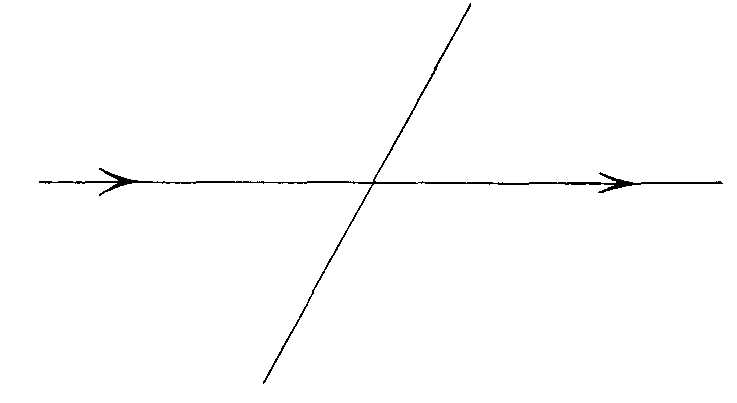
\includegraphics[width=70mm]{fig58.png}
\end{figure}

\begin{description}
\item{1.}~A straight line does not divide the plane. Starting from
the point of intersection of two lines and passing along one of them
a certain finite distance, we come to the intersection point again
without having crossed the other line. Thus, we can pass from one
side of the line to the other without having crossed it.

There is one point through which pass all the perpendiculars to a
given line. It is called the pole of that line, and the line is its
polar. Its distance from the line is half the entire length of a
straight line, and the line is the locus of points at this distance
from its pole. Therefore, if the pole of one line lies on another,
the pole of the second lies on the first, and the intersection of
two lines is the pole of the line joining their poles.

The locus of points at a given distance from a given line is a
circle having its centre at the pole of the line. The straight line
is a limiting form of a circle when the radius becomes equal to half
the entire length of a line.

We can draw three lines, each perpendicular to the other two,
forming a trirectangular triangle. It is also a self-polar triangle;
each vertex is the pole of the opposite side.

\item[2.]~All the perpendiculars to a plane in space meet at a point
which is the pole of the plane. It is the centre of a system of
spheres of which the plane is a limiting form when the radius
becomes equal to half the entire length of a straight line.

Figures on a plane can be projected from similar figures on any
sphere which has the pole of the plane for centre. That is, they
have equal angles and corresponding sides in a constant ratio that
depends only on the radius of the sphere. Two corresponding angles
are equal, because they are the same as the diedral angles formed by
the two planes through the centre of the sphere which cut the sphere
and the plane in the sides of the angles. Corresponding lines are
proportional; for if two arcs on the sphere are equal, their
projections on the plane are equal; and that, in general, two arcs
have the same ratio as their projections on the plane is proved,
first when they are commensurable, and by the method of limits when
they are incommensurable.

Geometry on a plane is, therefore, like Spherical Geometry, but the
plane corresponds to only half a sphere, just as the diameters of a
sphere correspond to the points of half the surface. Indeed, the
points and straight lines of a plane correspond exactly to the lines
and planes through a point, but we can realize the correspondence
better that compares the plane with the surface of a sphere. If we
can imagine that the points on the boundary of a hemisphere at
opposite extremities of diameters are coincident, the hemisphere
will correspond to the elliptic plane. There is no particular line
of the plane that plays the part of boundary. All lines of the plane
are alike; the plane is unbounded, but not infinite in extent.

The entire straight line corresponds to a semicircle. We will take
such a unit for measuring length that the entire length of a line
shall be $\pi$; the formulæ of Spherical Trigonometry will then
apply without change to our plane. Distances on a line will then
have the same measure as the angles which they subtend at the pole
of the line, and the angle between two lines will be equal to the
distance between their poles. The distance from any point to its
polar, half the entire length of a straight line, may then be called
a quadrant.

We can form a self-polar tetraëdron by taking three mutually
perpendicular planes and the plane which has their intersection for
pole. The vertices of this tetraëdron are the poles of the opposite
faces. At each vertex is a trirectangular triedral, and each face is
a trirectangular triangle.

\item[3.~Theorem.] \emph{All the planes perpendicular to a fixed line
intersect in another fixed line, called its polar or conjugate. The
relation is reciprocal, and all the points of either line are at a
quadrant's distance, from all the points of the other.}

\begin{figure}[h]
\centering
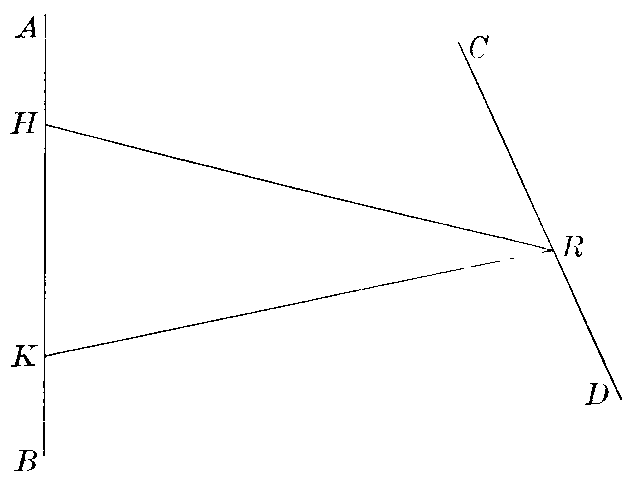
\includegraphics[width=60mm]{fig59.png}
\end{figure}

\textbf{Proof.} Let the two planes perpendicular to the line $AB$ at
$H$ and $K$ intersect in $CD$. Pass a plane through $AB$ and $R$,
any point of $CD$. This plane will intersect the two given planes in
$HR$ and $KR$. $HR$ and $KR$ are perpendicular to $AB$; therefore,
$R$ is at a quadrant's distance from $H$ and $K$. $R$ is then the
pole of $AB$ in the plane determined by $AR$ and $R$, and is at a
quadrant's distance from every point of $AB$. But $R$ is any point
of $CD$; therefore, any point of either line is at a quadrant's
distance from each point of the other line, and a point which is at
a quadrant's distance from one line lies in the other line. Again,
any point, $H$, of $AB$, being at a quadrant's distance from all the
points of $CD$, is the pole of $CD$ in the plane determined by it
and $CD$. Thus, $HR$ and $KR$ are both perpendicular to $CD$, and
the plane determined by $AB$ and $R$ is perpendicular to $CD$.

\medskip The opposite edges of a self-polar tetraëdron are polar
lines.

All the lines which intersect a given line at right angles intersect
its polar at right angles. Therefore, the distances of any point
from two polar lines are measured on the same straight line and are
together equal to a quadrant. Two points which are equidistant from
one line are equidistant from its polar.

The locus of points which are at a given distance from a fixed line
is a surface of revolution having both this line and its polar as
axes. We may call it a surface of double revolution. The parallel
circles about one axis are meridian curves for the other axis. If a
solid body, or, we may say, all space, move along a straight line
without rotating about it, it will rotate about the conjugate line
as an axis without sliding along it. A motion along a straight line
combined with a rotation about it is called a screw motion. A screw
motion may then be described as a rotation about each of two
conjugate lines or as a sliding along each of two conjugate lines.

\item[4.~Theorem.] \emph{In the elliptic geometry there are lines
not in the same plane which have an infinite number of common
perpendiculars and are everywhere equidistant.}

\begin{figure}[h]
\centering
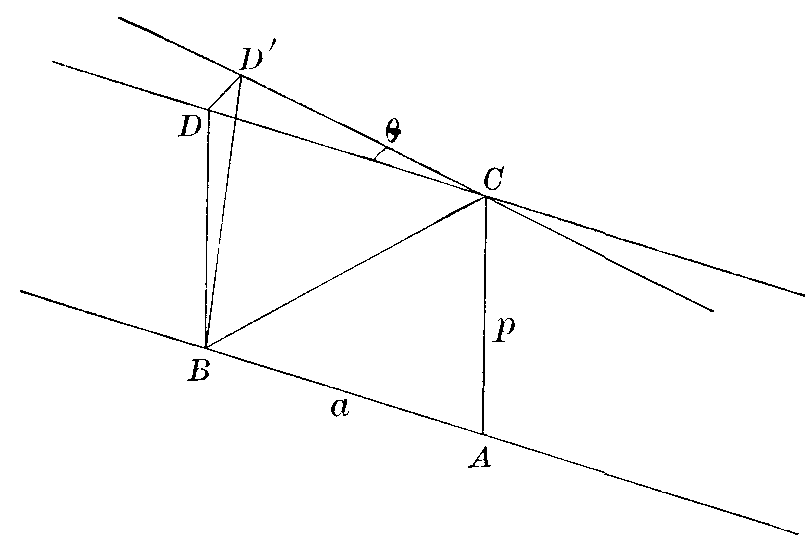
\includegraphics[width=80mm]{fig60.png}
\end{figure}

\textbf{Given} any two lines in the same plane and their common
perpendicular. If we go out on these lines in either direction from
the perpendicular, they approach each other. Now revolve one of them
about this perpendicular so that they are no longer in the same
plane. After a certain amount of rotation the lines will have an
infinite number of common perpendiculars and be equidistant
throughout their entire length.

\textbf{Proof.} Let $p$ be the length of the common perpendicular
$AC$, and take points $B$ and $D$ on the two lines on the same
side of this perpendicular at a distance, $a$.

$BD<p$, but if $CD$ revolve about $AC$, $BD$ will become longer than
$p$ by the time $CD$ is revolved through a right angle; for $BCD$
will then be a right triangle, with $BD$ for hypothenuse and $BC$,
the hypothenuse of the triangle $ABC$, for one of its sides, so that
we shall have $BD >BC$ and $BC > AC$.

Suppose, when $CD$ has revolved through an angle, $\theta$, $BD$
becomes equal to $p$ and takes the position $BD'$. The triangles
$ABC$ and $D'BC$ are equal, having corresponding sides equal.
Therefore, $BD'$ is perpendicular to $CD'$. $BD'$ is also
perpendicular to $BA$; for if we take the diedral $A-BC-D'$ and
place it upon itself so that the positions of $B$ and $C$ shall be
interchanged, $A$ will fall on the position of $D'$, and $D'$ on the
position of $A$, and the angle $D'BA$ must equal the angle $ACD'$.
Therefore, $BD'$ as well as $CA$ is a common perpendicular to the
lines $AB$ and $CD'$.

Now at the point $C$ we have a triedral whose three edges are $CB$,
$CD$, and $CD'$. Moreover, the diedral along the edge $CD$ is a
right diedral; therefore, the three face angles of the triedral
satisfy the same relations as do the three sides of a spherical
right triangle; namely,
\begin{gather*}
\cos BCD' = \cos BCD\, \cos DCD' \\
\intertext{But}
BCD = \frac{\pi}{2} - ACB \quad\text{and}\quad BCD' = ABC. \\
\intertext{Hence, this relation may be written}
\cos ABC = \sin ACB\, \cos \theta.
\end{gather*}

\P~Again, in the right triangle $ABC$
\begin{align*}
\sin ACB &= \frac{\cos ABC}{\cos p} \\
\therefore \cos \theta &= \cos p, \\
\intertext{or, since $\theta$ and $p$ are less than
$\nicefrac{\pi}{2}$,}
\theta &= p.
\end{align*}

The angle $\theta$, therefore, does not depend upon $a$. If we take
any two lines in a plane and turn one about their common
perpendicular through an angle equal in measure to the length of
that perpendicular, the two lines will then be everywhere
equidistant.
\end{description}

\label{p68ref}As we have no parallel lines in the ordinary sense in
this Geometry, the name \emph{parallel} has been applied to lines of
this kind. They have many properties of the parallel lines of
Euclidean Geometry.

Through any point two lines can be drawn parallel to a given line.
These are of two kinds, sometimes distinguished as right-wound and
left-wound. They lie entirely on a surface of double revolution,
having the given line as axis. The surface is, therefore, a ruled
surface and has on it two sets of rectilinear generators like the
hyperboloid of one sheet.

